\documentclass[11pt]{charter}

\usepackage{pdflscape}
\usepackage{tikz}
\usetikzlibrary{positioning}
\usepackage{pgfgantt}

% El títulos de la memoria, se usa en la carátula y se puede usar el cualquier lugar del documento con el comando \ttitle
\titulo{Software probador de relé ferroviario} 

% Nombre del posgrado, se usa en la carátula y se puede usar el cualquier lugar del documento con el comando \degreename
\posgrado{Carrera de Especialización en Sistemas Embebidos} 
%\posgrado{Carrera de Especialización en Internet de las Cosas} 
%\posgrado{Carrera de Especialización en Intelegencia Artificial}
%\posgrado{Maestría en Sistemas Embebidos} 
%\posgrado{Maestría en Internet de las cosas}

% Tu nombre, se puede usar el cualquier lugar del documento con el comando \authorname
\autor{Nicolás Locatelli} 

% El nombre del director y co-director, se puede usar el cualquier lugar del documento con el comando \supname y \cosupname y \pertesupname y \pertecosupname
\director{Gustavo Ramoscelli}
\pertenenciaDirector{GICSAFE} 
% FIXME:NO IMPLEMENTADO EL CODIRECTOR ni su pertenencia
\codirector{} % si queda vacio no se deberíá incluir 
\pertenenciaCoDirector{}

% Nombre del cliente, quien va a aprobar los resultados del proyecto, se puede usar con el comando \clientename y \empclientename
\cliente{Martín Harris}
\empresaCliente{Trenes Argentinos}

% Nombre y pertenencia de los jurados, se pueden usar el cualquier lugar del documento con el comando \jurunoname, \jurdosname y \jurtresname y \perteunoname, \pertedosname y \pertetresname.
\juradoUno{Nombre y Apellido (1)}
\pertenenciaJurUno{pertenencia (1)} 
\juradoDos{Nombre y Apellido (2)}
\pertenenciaJurDos{pertenencia (2)}
\juradoTres{Nombre y Apellido (3)}
\pertenenciaJurTres{pertenencia (3)}
 
\fechaINICIO{22 de junio de 2020}		%Fecha de inicio de la cursada de GdP \fechaInicioName
\fechaFINALPlanificacion{22 de Agosto de 2020} 	%Fecha de final de cursada de GdP
\fechaFINALTrabajo{22 de diciembre de 2020}		%Fecha de defensa pública del trabajo final


\begin{document}

\maketitle
\thispagestyle{empty}
\pagebreak


\thispagestyle{empty}
{\setlength{\parskip}{0pt}
\tableofcontents{}
}
\pagebreak


\section{Registros de cambios}
\label{sec:registro}


\begin{table}[ht]
\label{tab:registro}
\centering
\begin{tabularx}{\linewidth}{@{}|c|X|c|@{}}
\hline
\rowcolor[HTML]{C0C0C0} 
Revisión & \multicolumn{1}{c|}{\cellcolor[HTML]{C0C0C0}Detalles de los cambios realizados} & Fecha      \\ \hline
1.0      & Creación del documento                                          & 27/06/2020 \\ \hline
1.1      & Avance sobre puntos 1 a 6 del documento                                                               & 09/07/2020 \\ \hline
1.2      & Avance sobre puntos 7 a 12 del documento                                                               & 27/07/2020 \\ \hline
\end{tabularx}
\end{table}

\pagebreak



\section{Acta de Constitución del Proyecto}
\label{sec:acta}

\begin{flushright}
Buenos Aires, \fechaInicioName
\end{flushright}

\vspace{2cm}

Por medio de la presente se acuerda con el Ing. \authorname\hspace{1px} que su Trabajo Final de la \degreename\hspace{1px} se titulará ``\ttitle'', consistirá esencialmente en el prototipo preliminar de un sitio web para la configuración y muestra de resultados de los ensayos a realizar por el sistema probador de relés ferroviarios.
Tendrá un presupuesto preliminar estimado de 600 hs de trabajo y sin presupuesto asignado, con fecha de inicio \fechaInicioName\hspace{1px} y fecha de presentación pública \fechaFinalName.

Se adjunta a esta acta la planificación inicial.

\vfill

% Esta parte se construye sola con la información que hayan cargado en el preámbulo del documento y no debe modificarla
\begin{table}[ht]
\centering
\begin{tabular}{ccc}
\begin{tabular}[c]{@{}c@{}}Ariel Lutenberg \\ Director posgrado FIUBA\end{tabular} &  & \begin{tabular}[c]{@{}c@{}}\clientename \\ \empclientename \end{tabular} \vspace{2.5cm} \\ 
\multicolumn{3}{c}{\begin{tabular}[c]{@{}c@{}} \supname \\ Director del Trabajo Final\end{tabular}} \vspace{2.5cm} \\
\begin{tabular}[c]{@{}c@{}}\jurunoname \\ Jurado del Trabajo Final\end{tabular}     &  & \begin{tabular}[c]{@{}c@{}}\jurdosname\\ Jurado del Trabajo Final\end{tabular}  \vspace{2.5cm}  \\
\multicolumn{3}{c}{\begin{tabular}[c]{@{}c@{}} \jurtresname\\ Jurado del Trabajo Final\end{tabular}} \vspace{.5cm}                                                                     
\end{tabular}
\end{table}


\section{Descripción técnica-conceptual del Proyecto a realizar}
\label{sec:descripcion}

La organización CONICET-GICSAFe se caracteriza por su misión de realizar proyectos ferroviarios basados en electrónica e informática con alto impacto social y económico.

En el marco del proyecto '\title', este subproyecto tiene por finalidad la realización de una interfaz de usuario web, que permita al personal encargado de los ensayos aplicados a los relés ferroviarios, configurar fácilmente dichos ensayos y poder visualizar de forma resumida y clara los resultados de los mismos.

El presente proyecto se destaca  especialmente por ser el primero de su tipo en Argentina. No hay hasta el momento un emprendimiento destinado a la fabricación y prueba local de relés de tipo ferroviario.

En la Figura \ref{fig:diagBloques} se presenta el diagrama conceptual del sistema. El bloque resaltado en azul es la parte correspondiente al proyecto descripto en este documento. Se muestra la relación que tiene con el resto de las partes del sistema.

\vspace{25px}

\begin{figure}[htpb]
\centering 
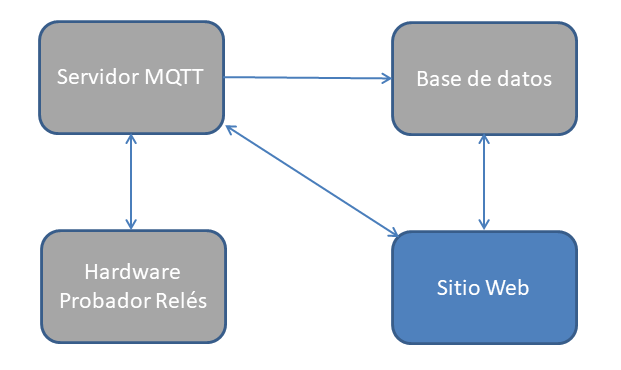
\includegraphics[width=.7\textwidth]{./Figuras/diagramaConceptual.png}
\caption{Diagrama conceptual del sistema}
\label{fig:diagBloques}
\end{figure}

\vspace{25px}

\newpage

\section{Identificación y análisis de los interesados}
\label{sec:interesados}

\begin{table}[ht]
%\caption{Identificación de los interesados}
%\label{tab:interesados}
\begin{tabularx}{\linewidth}{@{}|l|X|X|l|@{}}
\hline
\rowcolor[HTML]{C0C0C0} 
Rol           & Nombre y Apellido & Organización 	& Puesto 	\\ \hline
Cliente       & \clientename      &\empclientename	& -      	\\ \hline
Impulsor      & Mariano Fernandez Soler  & Trenes Argentinos   	& -        	\\ \hline
Responsable   & \authorname       & GICSAFE        	& Alumno 	\\ \hline
Orientador    & \supname	      & \pertesupname 	& Director Trabajo final \\ \hline
Colaborador    & Ariel Lutemberg  & GICSAFE 	& Director Posgrado \\ \hline
Equipo        & Gustavo Ramoscelli& GICSAFE        	& Docente        	\\ \hline
Usuario final & \clientename      &\empclientename 	& -       	\\ \hline
\end{tabularx}
\end{table}


\section{1. Propósito del proyecto}
\label{sec:proposito}

El propósito de este proyecto es implementar un sitio web para facilitar la configuración de los ensayos a realizar a cada relé y la representación gráfica de los
datos que surgen como resultado de los mismos.

\section{2. Alcance del proyecto}
\label{sec:alcance}

El presente proyecto incluye:
\begin{itemize}
\item Autenticación de usuarios mediante nombre de usuario y contraseña.
\item Esquema de autorización de usuarios mediante tres roles diferentes: administrador, configurador y usuario de sólo lectura.
\item Vista de configuración para los distintos tipos de ensayos (1, 2 y 3).
\item Vista de los resultados de cada ensayo realizado.
\item Persistencia de configuraciones y resultados en base de datos PostGres provista por el cliente.
\end{itemize}

El presente proyecto NO incluye:
\begin{itemize}
\item Nada por fuera de lo mencionado en el alcance.
\end{itemize}


\section{3. Supuestos del proyecto}
\label{sec:supuestos}

Para el desarrollo del presente proyecto se supone:

\begin{itemize}
\item Los requerimientos no sufrirán modificaciones de consideración durante la implementación del proyecto.
\item Disponer de los recursos necesarios (PC, acceso a internet, software utilizado) para realizar la tarea.
\item El cliente proveerá el hardware sobre el cuál se instalará el sitio web y la base de datos.
\end{itemize}


\section{4. Requerimientos}
\label{sec:requerimientos}

\begin{enumerate}
\item Grupo de requerimientos asociados con Usuarios:
	\begin{enumerate}
	\item Los usuarios del sistema deberán autenticarse para usarlo.
	\item Las contraseñas de usuario tendrán encriptación AES.
	\item Habrá tres (3) roles de usuarios: Administrador, Configurador y Usuario de solo lectura.
	\item Pantalla de login de usuario. Un usuario no autenticado será redirigido a esta pantalla.
	\item Un usuario Administrador solo podrá administrar usuarios.
	\item Un usuario Configurador podrá utilizar la funcionalidad relativa a configuración de ensayos. 
	\item Un usuario de solo lectura podrá utilizar la funcionalidad relativa a la visualización de resultados.
	\end{enumerate}
\item Grupo de requerimientos asociados con configuración de ensayos:
	\begin{enumerate}
	\item Pantalla de configuración de ensayo.
	\item La pantalla permitirá al usuario seleccionar el relé, indicar el tipo de ensayo y los parámetros del mismo.
	\end{enumerate}
\item Grupo de requerimientos asociados con visualización de ensayos:
	\begin{enumerate}
	\item Pantalla de listado índice de relés.
	\item Al seleccionar un relé del listado, se mostrará una pantalla de resultados de ensayos del relé.
	\item La pantalla de resultados de ensayos del relé mostrará los resultados de los ensayos en forma numérica y gráfica, buscando una facil interpretación por parte del usuario.
	\end{enumerate}
	
\end{enumerate}

\section{5. Entregables principales del proyecto}
\label{sec:entregables}

\begin{itemize}
\item Manual de usuario
\item Código fuente
\item Informe final
\end{itemize}

\section{6. Desglose del trabajo en tareas}
\label{sec:wbs}

\begin{enumerate}
\item Grupo de tareas de planificación
	\begin{enumerate}
	\item Leer documentación del proyecto. (48 hs)
	\item Reuniones con el equipo. (16 hs)
	\end{enumerate}

\item Grupo de tareas de preparación
	\begin{enumerate}
	\item Organizar herramientas de desarrollo. (16 hs)
	\item Generación del entorno y el repositorio. (16 hs)
	\end{enumerate}

\item Grupo de tareas relacionadas con el modelo
	\begin{enumerate}
	\item Definir entidades y sus relaciones. (16 hs)
	\item Crear las migraciones para generar las tablas. (8 hs)
	\item Crear seeders para las tablas. (8 hs)
	\item Crear servicio de acceso a base de datos. (16 hs)
	\item Crear API de acceso a datos. (16 hs)
	\item Verificación. (8 hs)
	\end{enumerate}

\item Grupo de tareas relacionadas con usuarios
	\begin{enumerate}
	\item Estudiar y agregar plugin de autenticación. (8 hs)
	\item Estudiar plugin de roles. (16 hs)
	\item Agregar plugin de roles y definir roles. (16 hs)
	\item Verificación. (8 hs)
	\end{enumerate}

\item Grupo de tareas relacionadas con el servidor Nodered
	\begin{enumerate}
	\item Implementar recepción e inserción de registros. (24 hs)
	\end{enumerate}

\item Grupo de tareas relacionadas con configuración de ensayos
	\begin{enumerate}
	\item Definir vistas de configuración. (16 hs)
	\item Implementar componentes Vue. (24 hs)
	\item Implementar vistas. (24 hs)
	\item Verificación. (8 hs)
	\end{enumerate}

\item Grupo de tareas relacionadas con visualización de ensayos
	\begin{enumerate}
	\item Estudiar Google Vue Charts. (8 hs)
	\item Diseñar vistas para cada tipo de ensayo. (16 hs)
	\item Implementar componente Vue para cada tipo. (48 hs)
	\item Verificación. (8 hs)
	\end{enumerate}

\item Grupo de tareas relacionadas con el area de hardware
	\begin{enumerate}
	\item Acordar estructuras de datos. (16 hs)
	\item Reuniones de asistencia e intercambio. (16 hs)
	\end{enumerate}

\item Grupo de tareas relacionadas con la aprobación
	\begin{enumerate}
	\item Realizar los tests de aprobación. (32 hs)
	\end{enumerate}

\end{enumerate}

Cantidad total de horas: (456 hs)



\section{7. Diagrama de Activity On Node}
\label{sec:AoN}

\begin{landscape}

\begin{tikzpicture}[
hito/.style={circle, draw=black, thick, minimum size=2cm},
tarea/.style={rectangle, draw=black, thick, minimum size=2cm, text width=2em, text centered},
]
%Nodes
\node[hito]      (inicio)                              	{Inicio};
\node[tarea]     (tarea_1_1)       [right=of inicio] 	{Tarea 1.1\\t=6d};
\node[tarea]     (tarea_1_2)       [below=of tarea_1_1] {Tarea 1.2\\t=2d};

\node[tarea]     (tarea_2_1)       [right=of tarea_1_2] {Tarea 2.1\\t=2d};
\node[tarea]     (tarea_2_2)       [right=of tarea_2_1] {Tarea 2.2\\t=2d};

\node[hito]      (empezar)		   [right=of tarea_2_2] {Listos};

\node[tarea]     (tarea_3_1)       [right=of empezar] 	{Tarea 3.1\\t=2d};
\node[tarea]     (tarea_3_2)       [right=of tarea_3_1] {Tarea 3.2\\t=1d};
\node[tarea]     (tarea_3_3)       [right=of tarea_3_2] 	{Tarea 3.3\\t=1d};
\node[tarea]     (tarea_3_4)       [below=of tarea_3_3] 	{Tarea 3.4\\t=2d};
\node[tarea]     (tarea_3_5)       [below=of tarea_3_4] 	{Tarea 3.5\\t=2d};
\node[tarea]     (tarea_3_6)       [right=of tarea_3_5] 	{Tarea 3.6\\t=1d};

\node[hito]      (modelo_listo)	   [right=of tarea_3_6] {Modelo listo};

\node[tarea]     (tarea_4_1)       [right=of modelo_listo] 	{Tarea 4.1\\t=1d};
\node[tarea]     (tarea_4_2)       [below=of tarea_4_1] 	{Tarea 4.2\\t=2d};
\node[tarea]     (tarea_4_3)       [right=of tarea_4_2] 	{Tarea 4.3\\t=2d};
\node[tarea]     (tarea_4_4)       [right=of tarea_4_3] 	{Tarea 4.4\\t=1d};

\node[tarea]     (tarea_5_1)       [below=of tarea_4_2] 	{Tarea 5.1\\t=3d};

\node[tarea]     (tarea_6_1)       [below=of tarea_5_1] 	{Tarea 6.1\\t=2d};
\node[tarea]     (tarea_6_2)       [right=of tarea_6_1] 	{Tarea 6.2\\t=3d};
\node[tarea]     (tarea_6_3)       [below=of tarea_6_2] 	{Tarea 6.3\\t=3d};
\node[tarea]     (tarea_6_4)       [right=of tarea_6_3] 	{Tarea 6.4\\t=1d};

\node[tarea]     (tarea_7_1)       [below=of tarea_6_3] 	{Tarea 7.1\\t=1d};
\node[tarea]     (tarea_7_2)       [right=of tarea_7_1] 	{Tarea 7.2\\t=2d};
\node[tarea]     (tarea_7_3)       [below=of tarea_7_2] 	{Tarea 7.3\\t=6d};
\node[tarea]     (tarea_7_4)       [right=of tarea_7_3] 	{Tarea 7.4\\t=1d};

\node[tarea]     (tarea_8_1)       [below=of tarea_3_1] 	{Tarea 8.1\\t=2d};
\node[tarea]     (tarea_8_2)       [right=of tarea_8_1] 	{Tarea 8.2\\t=2d};

\node[hito]      (implementado)	   [right=of tarea_7_4] {Implementado};

\node[tarea]     (tarea_9_1)       [right=of implementado] 	{Tarea 9.1\\t=4d};

\node[hito]      (fin)	   [right=of tarea_9_1] {Fin};

%Lines
\draw[->] (tarea_1_1.east) -- (tarea_1_2.west);

\end{tikzpicture}
\end{landscape}



\section{8. Diagrama de Gantt}
\label{sec:gantt}

%\begin{landscape}
\newpage

\begin{ganttchart}[
canvas/.append style={fill=none, draw=black!5, line width=.75pt},
hgrid style/.style={draw=black!5, line width=.75pt},
vgrid={*1{draw=black!5, line width=.75pt}},
today=1,
today rule/.style={
draw=black!64,
dash pattern=on 3.5pt off 4.5pt,
line width=1.5pt
},
today label font=\small\bfseries,
title/.style={draw=none, fill=none},
title label font=\bfseries\footnotesize,
title label node/.append style={below=7pt},
include title in canvas=false,
bar label font=\mdseries\small\color{black!70},
bar label node/.append style={left=2cm},
bar/.append style={draw=none, fill=black!63},
bar incomplete/.append style={fill=grey},
bar progress label font=\mdseries\footnotesize\color{black!70},
group incomplete/.append style={fill=blue},
group left shift=0,
group right shift=0,
group height=.3,
group peaks tip position=0,
group label node/.append style={left=.6cm},
group progress label font=\bfseries\small,
link/.style={-latex, line width=1pt, red},
link label font=\scriptsize\bfseries,
link label node/.append style={below left=-2pt and 0pt},
]{1}{120}

\gantttitle{Software probador de relés de tipo ferroviario}{120} \\[grid]
\gantttitle{Agosto}{30}
\gantttitle{Septiembre}{30}
\gantttitle{Octubre}{30}
\gantttitle{Noviembre}{30}\\
\gantttitle[
title label node/.append style={below left=7pt and -3pt}
]{Día:\quad1}{1}
\gantttitlelist{2,...,120}{1} \\
\ganttgroup[progress=0]{Planificación}{1}{8} \\
\ganttbar[
name=tarea_1_1
]{\textbf{Tarea 1.1}}{1}{6} \\
\ganttbar[
name=tarea_1_2
]{\textbf{Tarea 1.2}}{7}{8} \\

\ganttgroup[progress=0]{Preparación}{9}{12} \\
\ganttbar[
name=tarea_2_1
]{\textbf{Tarea 2.1}}{9}{10} \\
\ganttbar[
name=tarea_2_2
]{\textbf{Tarea 2.2}}{11}{12} \\

\ganttgroup[progress=0]{Modelo}{13}{18} \\
\ganttbar[
name=tarea_3_1
]{\textbf{Tarea 3.1}}{13}{14} \\
\ganttbar[
name=tarea_3_2
]{\textbf{Tarea 3.2}}{15}{15} \\
\ganttbar[
name=tarea_3_3
]{\textbf{Tarea 3.3}}{16}{16} \\
\ganttbar[
name=tarea_3_4
]{\textbf{Tarea 3.4}}{16}{17} \\
\ganttbar[
name=tarea_3_5
]{\textbf{Tarea 3.5}}{16}{17} \\
\ganttbar[
name=tarea_3_6
]{\textbf{Tarea 3.6}}{18}{18} \\

\ganttgroup[progress=0]{Usuarios}{19}{24} \\
\ganttbar[
name=tarea_4_1
]{\textbf{Tarea 4.1}}{19}{19} \\
\ganttbar[
name=tarea_4_2
]{\textbf{Tarea 4.2}}{20}{21} \\
\ganttbar[
name=tarea_4_3
]{\textbf{Tarea 4.3}}{22}{23} \\
\ganttbar[
name=tarea_4_4
]{\textbf{Tarea 4.4}}{24}{24} \\

\ganttgroup[progress=0]{Nodered}{19}{21} \\
\ganttbar[
name=tarea_5_1
]{\textbf{Tarea 5.1}}{19}{21} \\

\ganttgroup[progress=0]{Config ensayos}{19}{27} \\
\ganttbar[
name=tarea_6_1
]{\textbf{Tarea 6.1}}{19}{20} \\
\ganttbar[
name=tarea_6_2
]{\textbf{Tarea 6.2}}{21}{23} \\
\ganttbar[
name=tarea_6_3
]{\textbf{Tarea 6.3}}{24}{26} \\
\ganttbar[
name=tarea_6_4
]{\textbf{Tarea 6.4}}{27}{27} \\

\ganttgroup[progress=0]{Visualización ensayos}{19}{28} \\
\ganttbar[
name=tarea_7_1
]{\textbf{Tarea 7.1}}{19}{19} \\
\ganttbar[
name=tarea_7_2
]{\textbf{Tarea 7.2}}{20}{21} \\
\ganttbar[
name=tarea_7_3
]{\textbf{Tarea 7.3}}{22}{27} \\
\ganttbar[
name=tarea_7_4
]{\textbf{Tarea 7.4}}{28}{28} \\

\ganttgroup[progress=0]{Relación con hardware}{19}{23} \\
\ganttbar[
name=tarea_8_1
]{\textbf{Tarea 8.1}}{19}{20} \\
\ganttbar[
name=tarea_8_2
]{\textbf{Tarea 8.2}}{21}{22} \\

\ganttgroup[progress=0]{Tests de aprobación}{29}{33} \\
\ganttbar[
name=tarea_9_1
]{\textbf{Tarea 9.1}}{29}{33} \\

%Links
\ganttlink{tarea_1_1}{tarea_1_2}
\ganttlink{tarea_1_2}{tarea_2_1}
\ganttlink{tarea_2_1}{tarea_2_2}

\ganttlink{tarea_2_2}{tarea_3_1}
\ganttlink{tarea_3_1}{tarea_3_2}
\ganttlink{tarea_3_2}{tarea_3_3}
\ganttlink{tarea_3_2}{tarea_3_4}
\ganttlink{tarea_3_2}{tarea_3_5}
\ganttlink{tarea_3_5}{tarea_3_6}

\ganttlink{tarea_3_6}{tarea_4_1}
\ganttlink{tarea_4_1}{tarea_4_2}
\ganttlink{tarea_4_2}{tarea_4_3}
\ganttlink{tarea_4_3}{tarea_4_4}

\ganttlink{tarea_3_6}{tarea_5_1}

\ganttlink{tarea_3_6}{tarea_6_1}

\ganttlink{tarea_3_6}{tarea_7_1}

\ganttlink{tarea_3_1}{tarea_8_1}

\ganttlink{tarea_7_4}{tarea_9_1}
\ganttlink{tarea_6_4}{tarea_9_1}
\ganttlink{tarea_4_4}{tarea_9_1}

\end{ganttchart}

%\end{landscape}


\section{9. Matriz de uso de recursos de materiales}
\label{sec:recursos}


\begin{table}[htpb]
\label{tab:recursos}
\centering
\begin{tabular}{|l|l|c|c|c|}
\hline
\multicolumn{1}{|c|}{\multirow{2}{*}{\begin{tabular}[c]{@{}c@{}}Código\\ WBS\end{tabular}}} & \multicolumn{1}{c|}{\multirow{2}{*}{Nombre tarea}} & \multicolumn{3}{c|}{Uso de recursos [hs]} \\ \cline{3-5} 
\multicolumn{1}{|c|}{}                                                                      & \multicolumn{1}{c|}{}                              & Notebook 1 & Notebook 2 & Servidor \\ \hline

1.1 & Leer documentación del proyecto  & 48 &  &  \\ \hline
1.2 & Reuniones con el equipo & 16 &  &  \\ \hline
2.1 & Organizar herramientas de desarrollo & 16 &  & 8 \\ \hline
2.2 & Generación del entorno y el repositorio & 16 &  & 8 \\ \hline
3.1 & Definir entidades y sus relaciones & 16 &  &  \\ \hline
3.2 & Crear las migraciones para generar las tablas & 8 &  &  \\ \hline
3.3 & Crear Seeders para las tablas & 8 &  &  \\ \hline
3.4 & Crear servicio de acceso a base de datos & 16 &  &  \\ \hline
3.5 & Crear API de acceso a datos & 16 &  &  \\ \hline
3.6 & Verificación & 8 &  &  \\ \hline
4.1 & Estudiar y agregar plugin de autenticación & 8 &  &  \\ \hline
4.2 & Estudiar plugin de roles & 16 &  &  \\ \hline
4.3 & Agregar plugin de roles y definir roles & 16 &  &  \\ \hline
4.4 & Verificación & 8 &  &  \\ \hline
5.1 & Implementar recepción e inserción de registros & 24 &  & 24 \\ \hline
6.1 & Definir vistas de configuración & 16 &  &  \\ \hline
6.2 & Implementar componentes Vue & 24 &  &  \\ \hline
6.3 & Implementar vistas & 24 &  &  \\ \hline
6.4 & Verificación & 8 &  &  \\ \hline
7.1 & Estudiar Google Vue Charts & 8 &  &  \\ \hline
7.2 & Diseñar vistas para cada tipo de ensayo & 16 &  &  \\ \hline
7.3 & Implementar componente Vue para cada tipo & 48 &  &  \\ \hline
7.4 & Verificación & 8 &  &  \\ \hline
8.1 & Acordar estructuras de datos & 16 &  &  \\ \hline
8.2 & Reuniones de asistencia e intercambio & 16 &  &  \\ \hline
9.1 & Realizar los tests de aprobación & 32 &  & 32 \\ \hline
\end{tabular}
\end{table}


\section{10. Presupuesto detallado del proyecto}
\label{sec:presupuesto}

\begin{consigna}{red}
Si el proyecto es complejo entonces separarlo en partes:
\begin{itemize}
\item Un total global, indicando el subtotal acumulado por cada una de las áreas.
\item El desglose detallado del subtotal de cada una de las áreas.
\end{itemize}

IMPORTANTE: No olvidarse de considerar los COSTOS INDIRECTOS.

\end{consigna}

\begin{table}[htpb]
\centering
\begin{tabularx}{\linewidth}{@{}|X|c|r|r|@{}}
\hline
\rowcolor[HTML]{C0C0C0} 
\multicolumn{4}{|c|}{\cellcolor[HTML]{C0C0C0}COSTOS DIRECTOS} \\ \hline
\rowcolor[HTML]{C0C0C0} 
Descripción &
  \multicolumn{1}{c|}{\cellcolor[HTML]{C0C0C0}Cantidad} &
  \multicolumn{1}{c|}{\cellcolor[HTML]{C0C0C0}Valor unitario} &
  \multicolumn{1}{c|}{\cellcolor[HTML]{C0C0C0}Valor total} \\ \hline
 &
  \multicolumn{1}{c|}{} &
  \multicolumn{1}{c|}{} &
  \multicolumn{1}{c|}{} \\ \hline
 &
  \multicolumn{1}{c|}{} &
  \multicolumn{1}{c|}{} &
  \multicolumn{1}{c|}{} \\ \hline
\multicolumn{1}{|l|}{} &
   &
   &
   \\ \hline
\multicolumn{1}{|l|}{} &
   &
   &
   \\ \hline
\multicolumn{3}{|c|}{SUBTOTAL} &
  \multicolumn{1}{c|}{} \\ \hline
\rowcolor[HTML]{C0C0C0} 
\multicolumn{4}{|c|}{\cellcolor[HTML]{C0C0C0}COSTOS INDIRECTOS} \\ \hline
\rowcolor[HTML]{C0C0C0} 
Descripción &
  \multicolumn{1}{c|}{\cellcolor[HTML]{C0C0C0}Cantidad} &
  \multicolumn{1}{c|}{\cellcolor[HTML]{C0C0C0}Valor unitario} &
  \multicolumn{1}{c|}{\cellcolor[HTML]{C0C0C0}Valor total} \\ \hline
\multicolumn{1}{|l|}{} &
   &
   &
   \\ \hline
\multicolumn{1}{|l|}{} &
   &
   &
   \\ \hline
\multicolumn{1}{|l|}{} &
   &
   &
   \\ \hline
\multicolumn{3}{|c|}{SUBTOTAL} &
  \multicolumn{1}{c|}{} \\ \hline
\rowcolor[HTML]{C0C0C0}
\multicolumn{3}{|c|}{TOTAL} &
   \\ \hline
\end{tabularx}%
\end{table}


\section{11. Matriz de asignación de responsabilidades}
\label{sec:responsabilidades}
\begin{consigna}{red}
Establecer la matriz de asignación de responsabilidades y el manejo de la autoridad completando la siguiente tabla:

\begin{table}[htpb]
\centering
\resizebox{\textwidth}{!}{%
\begin{tabular}{|c|c|c|c|c|c|}
\hline
\rowcolor[HTML]{C0C0C0} 
\cellcolor[HTML]{C0C0C0} &
  \cellcolor[HTML]{C0C0C0} &
  \multicolumn{4}{c|}{\cellcolor[HTML]{C0C0C0}Listar todos los nombres y roles del proyecto} \\ \cline{3-6} 
\rowcolor[HTML]{C0C0C0} 
\cellcolor[HTML]{C0C0C0} &
  \cellcolor[HTML]{C0C0C0} &
  Responsable &
  Orientador &
  Equipo &
  Cliente \\ \cline{3-6} 
\rowcolor[HTML]{C0C0C0} 
\multirow{-3}{*}{\cellcolor[HTML]{C0C0C0}\begin{tabular}[c]{@{}c@{}}Código\\ WBS\end{tabular}} &
  \multirow{-3}{*}{\cellcolor[HTML]{C0C0C0}Nombre de la tarea} &
  \authorname &
  \supname &
  Nombre de alguien &
  \clientename \\ \hline
 &  &  &  &  &  \\ \hline
 &  &  &  &  &  \\ \hline
 &  &  &  &  &  \\ \hline
\end{tabular}%
}
\end{table}

{\footnotesize
Referencias:
\begin{itemize}
	\item P = Responsabilidad Primaria
	\item S = Responsabilidad Secundaria
	\item A = Aprobación
	\item I = Informado
	\item C = Consultado
\end{itemize}
} %footnotesize

Una de las columnas debe ser para el Director, ya que se supone que participará en el proyecto.
A su vez se debe cuidar que no queden muchas tareas seguidas sin ``A'' o ``I''.

Importante: es redundante poner ``I/A'' o ``I/C'', porque para aprobarlo o responder consultas primero la persona debe ser informada.

\end{consigna}

\section{12. Gestión de riesgos}
\label{sec:riesgos}

\begin{consigna}{red}
a) Identificación de los riesgos (al menos cinco) y estimación de sus consecuencias:
 
Riesgo 1: detallar el riesgo (riesgo es algo que si ocurre altera los planes previstos)
\begin{itemize}
\item Severidad (S): mientras más severo, más alto es el número (usar números del 1 al 10).\\
Justificar el motivo por el cual se asigna determinado número de severidad (S).
\item Probabilidad de ocurrencia (O): mientras más probable, más alto es el número (usar del 1 al 10).\\
Justificar el motivo por el cual se asigna determinado número de (O). 
\end{itemize}   

Riesgo 2:
\begin{itemize}
\item Severidad (S): 
\item Ocurrencia (O):
\end{itemize}

Riesgo 3:
\begin{itemize}
\item Severidad (S): 
\item Ocurrencia (O):
\end{itemize}


b) Tabla de gestión de riesgos:      (El RPN se calcula como RPN=SxO)

\begin{table}[htpb]
\centering
\begin{tabularx}{\linewidth}{@{}|X|c|c|c|c|c|c|@{}}
\hline
\rowcolor[HTML]{C0C0C0} 
Riesgo & S & O & RPN & S* & O* & RPN* \\ \hline
       &   &   &     &    &    &      \\ \hline
       &   &   &     &    &    &      \\ \hline
       &   &   &     &    &    &      \\ \hline
       &   &   &     &    &    &      \\ \hline
       &   &   &     &    &    &      \\ \hline
\end{tabularx}%
\end{table}

Criterio adoptado: 
Se tomarán medidas de mitigación en los riesgos cuyos números de RPN sean mayores a ....

Nota: los valores marcados con (*) en la tabla corresponden luego de haber aplicado la mitigación.

c) Plan de mitigación de los riesgos que originalmente excedían el RPN máximo establecido:
 
Riesgo 1: Plan de mitigación (si por el RPN fuera necesario elaborar un plan de mitigación).
  Nueva asignación de S y O, con su respectiva justificación:
  - Severidad (S): mientras más severo, más alto es el número (usar números del 1 al 10).
          Justificar el motivo por el cual se asigna determinado número de severidad (S).
  - Probabilidad de ocurrencia (O): mientras más probable, más alto es el número (usar del 1 al 10).
          Justificar el motivo por el cual se asigna determinado número de (O).

Riesgo 2: Plan de mitigación (si por el RPN fuera necesario elaborar un plan de mitigación).
 
Riesgo 3: Plan de mitigación (si por el RPN fuera necesario elaborar un plan de mitigación)

\end{consigna}


\section{13. Gestión de la calidad}
\label{sec:calidad}

\begin{consigna}{red}
Para cada uno de los requerimientos del proyecto indique:
\begin{itemize} 
\item Req \#1: Copiar acá el requerimiento.

Verificación y validación:

\begin{itemize}
\item Verificación para confirmar si se cumplió con lo requerido antes de mostrar el sistema al cliente:\\
Detallar 
\item Validación con el cliente para confirmar que está de acuerdo en que se cumplió con lo requerido:\\
Detallar  
\end{itemize}

\end{itemize}

Tener en cuenta que en este contexto se pueden mencionar simulaciones, cálculos, revisión de hojas de datos, consulta con expertos, etc.

\end{consigna}

\section{14. Comunicación del proyecto}
\label{sec:comunicaciones}

\begin{consigna}{red}
El plan de comunicación del proyecto es el siguiente:
\end{consigna}

% Please add the following required packages to your document preamble:
% \usepackage{graphicx}
% \usepackage[table,xcdraw]{xcolor}
% If you use beamer only pass "xcolor=table" option, i.e. \documentclass[xcolor=table]{beamer}
\begin{table}[htpb]
\centering
\resizebox{\textwidth}{!}{%
\begin{tabular}{|c|c|c|c|c|c|}
\hline
\rowcolor[HTML]{C0C0C0} 
\multicolumn{6}{|c|}{\cellcolor[HTML]{C0C0C0}PLAN DE COMUNICACIÓN DEL PROYECTO}           \\ \hline
\rowcolor[HTML]{C0C0C0} 
¿Qué comunicar? & Audiencia & Propósito & Frecuencia & Método de comunicac. & Responsable \\ \hline
                &           &           &            &                      &             \\ \hline
                &           &           &            &                      &             \\ \hline
                &           &           &            &                      &             \\ \hline
                &           &           &            &                      &             \\ \hline
                &           &           &            &                      &             \\ \hline
\end{tabular}%
}
\end{table}

\section{15. Gestión de Compras}
\label{sec:compras}

\begin{consigna}{red}
En caso de tener que comprar elementos o contratar servicios:
a) Explique con qué criterios elegiría a un proveedor.
b) Redacte el Statement of Work correspondiente.
\end{consigna}

\section{16. Seguimiento y control}
\label{sec:seguimiento}

\begin{consigna}{red}
Para cada tarea del proyecto establecer la frecuencia y los indicadores con los se seguirá su avance y quién será el responsable de hacer dicho seguimiento y a quién debe comunicarse la situación (en concordancia con el Plan de Comunicación del proyecto).

El indicador de avance tiene que ser algo medible, mejor incluso si se puede medir en \% de avance. Por ejemplo,se pueden indicar en esta columna cosas como ``cantidad de conexiones ruteadeas'' o ``cantidad de funciones implementadas'', pero no algo genérico y ambiguo como ``\%'', porque el lector no sabe porcentaje de qué cosa.

\end{consigna}

\begin{table}[!htpb]
\centering
\begin{tabularx}{\linewidth}{@{}|X|X|X|X|X|X|@{}}
\hline
\rowcolor[HTML]{C0C0C0} 
\multicolumn{6}{|c|}{\cellcolor[HTML]{C0C0C0}SEGUIMIENTO DE AVANCE}                                                                       \\ \hline
\rowcolor[HTML]{C0C0C0} 
Tarea del WBS & Indicador de avance & Frecuencia de reporte & Resp. de seguimiento & Persona a ser informada & Método de comunic. \\ \hline
 &  &  &  &  &  \\ \hline
 &  &  &  &  &  \\ \hline
 &  &  &  &  &  \\ \hline
 &  &  &  &  &  \\ \hline
 &  &  &  &  &  \\ \hline
\end{tabularx}%
%}
\end{table}

\section{17. Procesos de cierre}    
\label{sec:cierre}

\begin{consigna}{red}
Establecer las pautas de trabajo para realizar una reunión final de evaluación del proyecto, tal que contemple las siguientes actividades:

\begin{itemize}
\item Pautas de trabajo que se seguirán para analizar si se respetó el Plan de Proyecto original:
 - Indicar quién se ocupará de hacer esto y cuál será el procedimiento a aplicar. 
\item Identificación de las técnicas y procedimientos útiles e inútiles que se utilizaron, y los problemas que surgieron y cómo se solucionaron:
 - Indicar quién se ocupará de hacer esto y cuál será el procedimiento para dejar registro.
\item Indicar quién organizará el acto de agradecimiento a todos los interesados, y en especial al equipo de trabajo y colaboradores:
  - Indicar esto y quién financiará los gastos correspondientes.
\end{itemize}

\end{consigna}


\end{document}
